\documentclass[11pt,a4paper]{article}
\usepackage[margin=2.2cm]{geometry}
\usepackage{graphicx}
\usepackage{booktabs}
\usepackage{amsmath}
\usepackage{xcolor}
\usepackage[hidelinks]{hyperref}
\usepackage{caption}
\usepackage{float}
\captionsetup{font=small,labelfont=bf}
\setlength{\parskip}{0.45em}
\setlength{\parindent}{0pt}
\setlength{\emergencystretch}{2em}
% plain \input is not expandable inside a tabular, the primitive one is
\makeatletter\let\tabin\@@input\makeatother

\title{Text-Based Emotion Classification on GoEmotions:\\Distilling a Large Encoder into the Browser}
\author{Manas Pandya\\[0.2em]\small NLP \& CV Lab, Task 06}
\date{October 2026}

\begin{document}
\maketitle

\begin{center}
\small
Live demo: \url{https://nlp-cv-lab.vercel.app/p/emotion-classification}\\
Code: \url{https://github.com/manasrpandya/NLP_CV_Lab/tree/main/projects/06-emotion-classification}\\
Models: \url{https://huggingface.co/manasrpandya/goemotions-distil-onnx},
\url{https://huggingface.co/manasrpandya/goemotions-teacher}
\end{center}

\section{Aim}

The task is to classify the emotion expressed in a piece of text with a deep learning model. The common way
to do this is to fine-tune a BERT-style model on a six-class Twitter dataset (dair-ai/emotion) and report
accuracy, which ends up around 93\%. I wanted a harder setting that is closer to how emotion actually shows
up in text, so I used GoEmotions \cite{goemotions}: 27 fine-grained emotions plus neutral, where a comment can
carry several of them at once. That makes it a multi-label problem with very imbalanced labels (grief has 77
training examples, neutral has 14k).

The goals were:
\begin{enumerate}
\itemsep0em
\item[(a)] build a ladder of models, from a linear baseline and a recurrent network up to a large transformer,
and evaluate all of them the same way;
\item[(b)] get a small model that is close to the large one but small enough to run inside a web browser;
\item[(c)] make the probabilities it outputs mean something (calibration);
\item[(d)] check how well it transfers to a different domain (tweets) without any extra training;
\item[(e)] build a demo that is useful for poking at the model, with a per-word explanation and an
``emotion arc'' view for longer text.
\end{enumerate}

\section{Background}

\textbf{GoEmotions.} Demszky et al.\ \cite{goemotions} collected 58k Reddit comments, each labelled by three
or more raters with any subset of 27 emotions or neutral. The ``simplified'' release keeps the labels at least
two raters agreed on. Their BERT-base baseline gets 0.46 macro-F1 on the test set. They also group the labels
into Ekman's six basic emotions \cite{ekman} plus neutral, where BERT gets 0.64.

\textbf{Multi-label classification.} Each label gets its own sigmoid output and binary cross-entropy (BCE)
loss. The decision threshold does not have to be 0.5. For rare labels the model is rarely confident, so a
lower threshold picked on the validation set usually gives a much better F1. Asymmetric loss (ASL)
\cite{asl} is a variant of focal loss for multi-label problems that down-weights the many easy negatives more
than the positives.

\textbf{Knowledge distillation} \cite{hinton} trains a small student to match the softened outputs of a large
teacher as well as the gold labels. For sigmoid outputs I used the binary version: BCE between
$\sigma(z_s/T)$ and $\sigma(z_t/T)$, scaled by $T^2$.

\textbf{Calibration.} A classifier is calibrated if, among all the times it says 70\%, the label is actually
present about 70\% of the time. Expected calibration error (ECE) measures the gap with binned predictions.
Temperature scaling \cite{guo} divides all logits by one scalar fitted on validation data. It does not change
the ranking of any label, so F1 at tuned thresholds is unaffected.

\section{Data}

\begin{table}[H]
\centering\small
\begin{tabular}{lrrr}
\toprule
Dataset & Train & Val & Test \\
\midrule
GoEmotions simplified (Reddit, 28 labels, multi-label) & 43\,410 & 5\,426 & 5\,427 \\
dair-ai/emotion (Twitter, 6 classes, single label), OOD test only & -- & -- & 2\,000 \\
\bottomrule
\end{tabular}
\caption{Datasets. Only the official splits are used.}
\end{table}

GoEmotions comments are short (12.8 words on average) and 16\% of training comments have more than one label.
Names and religions are masked as \texttt{[NAME]} and \texttt{[RELIGION]}. The label distribution is extremely
skewed: neutral appears in a third of the comments, while grief, pride, relief and nervousness each have fewer
than 170 training examples and only 6--23 test examples, so their test F1 is noisy.

For the out-of-domain (OOD) test both label sets are mapped to Ekman groups. dair-ai/emotion has sadness, joy,
love, anger, fear and surprise; love goes into joy (GoEmotions also puts love under joy). It has no disgust and
no neutral, so the GoEmotions model's Ekman probabilities are restricted to the five shared groups and the
argmax is compared with the gold class. The Twitter text is lowercased with punctuation stripped, which is quite
different from Reddit, and none of it was used for training or tuning.

\section{Method}

\subsection{Models}

\textbf{TF-IDF + logistic regression.} Word 1--2 grams and character 2--5 grams (up to 200k features each,
sublinear TF), one class-balanced logistic regression per label. $C$ was picked from $\{1, 4, 16\}$ on
validation ($C=1$).

\textbf{BiGRU + GloVe.} A regex tokenizer, 300-d GloVe 6B vectors \cite{glove} for every word that has one
(22.7k of the 23.5k vocabulary, random init for the rest), a single bidirectional GRU with 256 units per
direction, max and mean pooling over time and a linear layer. The embeddings are fine-tuned with a 10$\times$
smaller learning rate. This is the classic ``deep learning before transformers'' baseline.

\textbf{Teachers: RoBERTa-large} \cite{roberta} (355M parameters) with the standard classification head over
the \texttt{<s>} token. I trained two, one with plain BCE and one with ASL ($\gamma_-=4$, $\gamma_+=0$,
clip 0.05). Both use AdamW with peak learning rate $2\cdot10^{-5}$, 6\% warmup and linear decay, layer-wise
learning rate decay (LLRD) of 0.95 per layer going down (so the embeddings get about $0.28\times$ the head's
rate), batch size 32, 4 epochs and fp16 mixed precision. The epoch with the best validation macro-F1 is kept.

\textbf{Student: DistilRoBERTa-base} \cite{distilbert} (82M parameters, 6 layers). I picked it over MiniLM
because it uses the same byte-level BPE tokenizer as RoBERTa, which keeps casing and emojis instead of
mapping them to \texttt{[UNK]}, and after int8 quantization it fits the roughly 90\,MB budget for the browser.
It is trained for 6 epochs at learning rate $6\cdot10^{-5}$ with LLRD 0.9 and the loss
\[
  \mathcal{L} = \alpha\,\mathrm{BCE}(z_s, y) + (1-\alpha)\,T^2\,\mathrm{BCE}\big(z_s/T,\ \sigma(\bar z_t/T)\big),
  \qquad \alpha = 0.5,\ T = 2,
\]
where $\bar z_t$ is the mean of the two teachers' logits on the training set. As an ablation, the same student
is also trained on hard labels only.

\subsection{Decision Rule and Calibration}
\label{sec:thr}

The same post-processing is applied to every model so the comparison is fair. On the validation set I fit one
temperature $T$ (grid search on the BCE), then pick a threshold per label between 0.02 and 0.95 that maximises
that label's F1. If no label passes its threshold, the one closest to it (highest $p/t$) is predicted, since
every GoEmotions comment has at least one label. Ekman scores are the maximum over each group's members, with
their own thresholds tuned the same way.

My first version took the plain argmax of each label's F1-versus-threshold curve. That turned out to be
unstable for rare labels: the int8 model, whose logits correlate 0.997 with the fp32 model's, got thresholds
of 0.27 instead of 0.64 for realization and a grief F1 of 0.55 instead of 0.18, and its test macro-F1 came out
0.026 higher than the fp32 model's. A quantized model is not really better, the curve just has narrow noisy
peaks (grief has 13 validation positives). I now smooth each curve with a 9-point moving average (a window of
$\pm0.04$) before taking the argmax, which halved that gap. All numbers below use the smoothed version.

ECE is computed over every (comment, label) pair with 15 bins. Because about 88\% of those pairs are easy
negatives below 0.05, this number is small for every model, so Table~\ref{tab:ece} also reports ECE restricted
to pairs where the model gives more than 5\%, which is the range the demo actually shows.

\subsection{Export}

The student is exported with Optimum \cite{optimum} to ONNX (opset 17), then quantized with ONNX Runtime's
dynamic int8 quantization (MatMul and Gather, so the 50k$\times$768 embedding matrix is int8 as well). An fp16
copy is made for WebGPU. Parity with PyTorch is checked with \texttt{labcore.parity} and the int8 model is
re-evaluated on the full test set. The browser uses the int8 model's own temperature and thresholds.

\subsection{Compute}

The transformers were trained on a free Colab T4 (fp16 only, no bf16), driven from the command line. One
RoBERTa-large epoch takes about 7 minutes (3.35 it/s), and the whole queue (two teachers, two students, the
BiGRU) took about 75 minutes of GPU time. Each run pushes its weights and logits to the Hugging Face Hub as
soon as it finishes. That paid off: the first VM was reclaimed after the two teachers, and a second one later
went idle and was reclaimed too, but the queue skips runs that are already on the Hub, so nothing had to be
retrained. Everything after training (TF-IDF, evaluation, export, benchmarks, figures) ran on a laptop CPU.

\section{Experiments and Results}

\subsection{Main Results}

\begin{table}[H]
\centering\footnotesize\setlength{\tabcolsep}{4.5pt}
\begin{tabular}{lrrrrrrr}
\toprule
& \multicolumn{3}{c}{GoEmotions, 28 labels} & Ekman & \multicolumn{2}{c}{OOD Twitter} & \\
\cmidrule(lr){2-4}\cmidrule(lr){6-7}
Model & Macro-F1 & Micro-F1 & Macro@0.5 & Macro-F1 & Acc & Macro-F1 & MB \\
\midrule
\tabin tables/main.tex 
\midrule
BERT-base \cite{goemotions} & 0.46 & -- & -- & 0.64 & -- & -- & -- \\
\bottomrule
\end{tabular}
\caption{Test results. Macro-F1 and micro-F1 use per-label thresholds tuned on validation; Macro@0.5 uses a
fixed 0.5 threshold. MB is the size of the weights on disk.}
\label{tab:main}
\end{table}

Table~\ref{tab:main} is the main result. Every transformer lands between 0.52 and 0.55 macro-F1, well above the
0.46 of the original paper and in the range of the best published numbers for this dataset. Even the TF-IDF
baseline reaches 0.47, which says more about the tuned thresholds than about TF-IDF: with a fixed 0.5 threshold
it gets 0.46, and most transformers lose 0.02--0.04 as well (the ensemble is the exception, its averaged
probabilities happen to sit around 0.5 already).

Because the rare labels make the test score noisy, I computed 95\% bootstrap intervals (500 resamples of the
test comments) and paired bootstrap differences (1000 resamples, the same comments for both models). The
intervals are about $\pm0.02$ wide, for example $[0.512, 0.552]$ for the student. The paired comparisons
give the following:
\begin{itemize}
\itemsep0em
\item Distillation helps: KD student minus hard-label student is $+0.014$ $[+0.002, +0.026]$, and micro-F1
goes up by 0.019. On validation the gap was even clearer (0.560 vs 0.539, Figure~\ref{fig:curves}).
\item The deployed int8 student and the teacher ensemble are not distinguishable: $+0.004$ $[-0.008, +0.017]$.
\item BCE vs ASL for the teacher makes no real difference in F1: $+0.005$ $[-0.011, +0.020]$.
\item Transformers clearly beat the recurrent baseline (hard-label student minus BiGRU: $+0.038$), while the
BiGRU is only marginally better than TF-IDF ($+0.013$ $[-0.003, +0.030]$).
\item The int8 row is $+0.009$ above the fp32 student with $p<0.01$. This is the threshold effect from
Section~\ref{sec:thr} again: the bootstrap only resamples the test set, not the threshold selection. With the fp32
model's thresholds, quantization changes test macro-F1 from 0.5338 to 0.5325.
\end{itemize}

\subsection{Per-Label Results}

\begin{figure}[H]
\centering
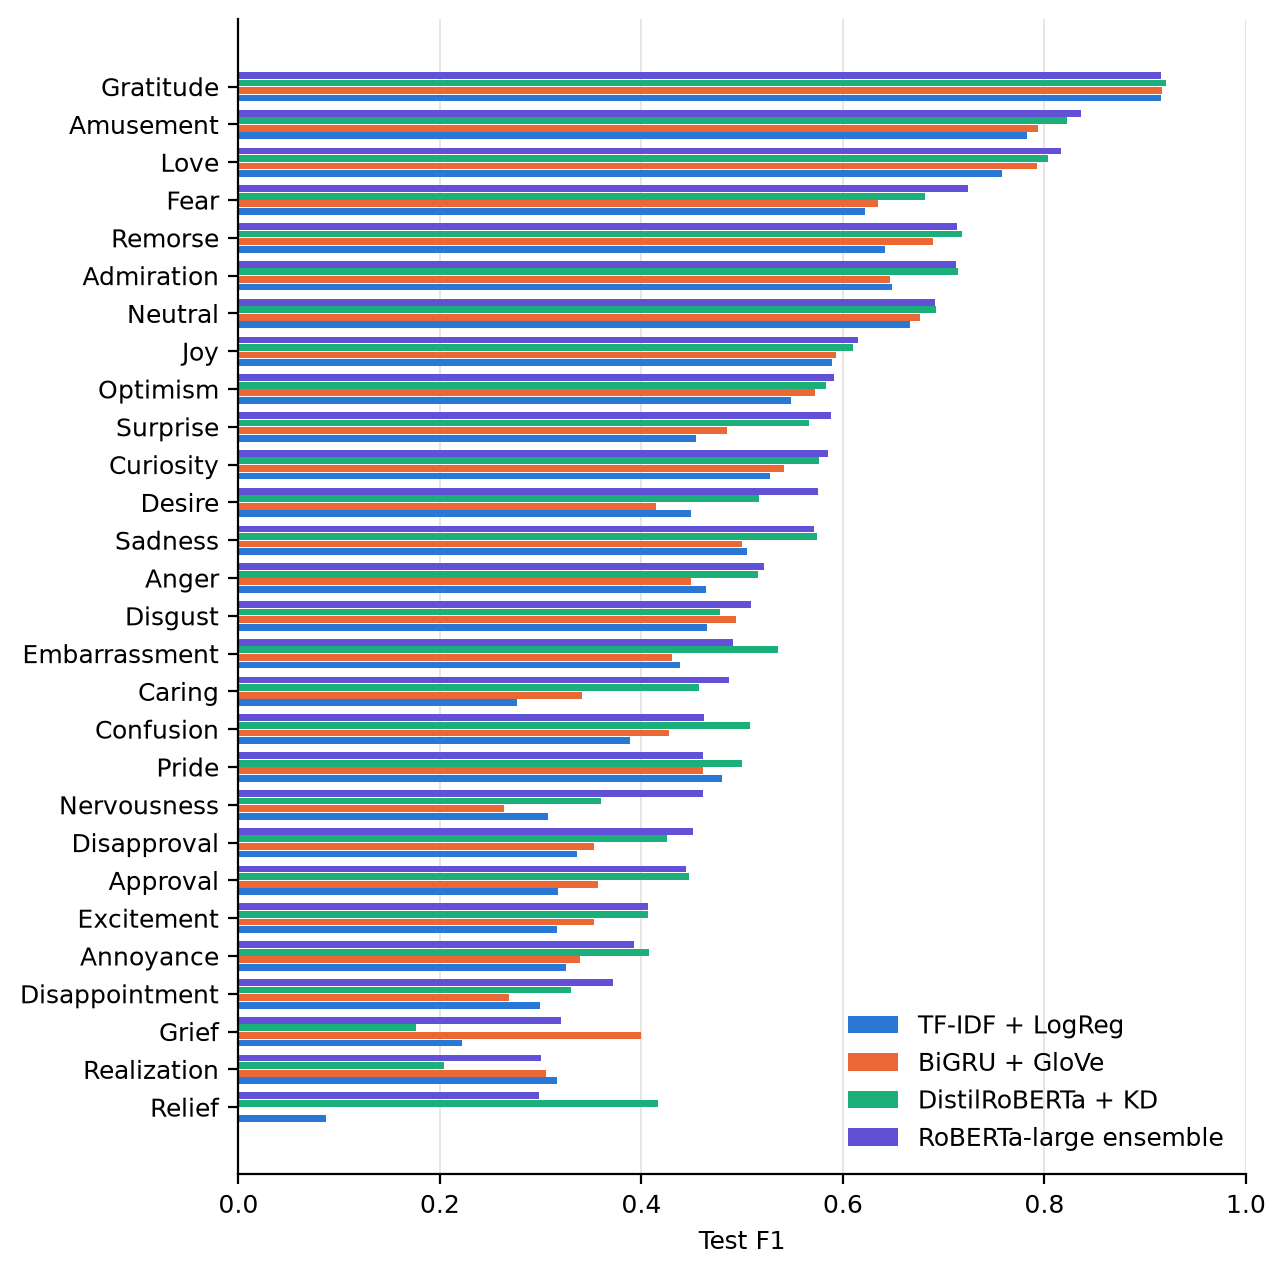
\includegraphics[width=0.72\linewidth]{figs/per_label_f1.png}
\caption{Per-label test F1, sorted by the teacher ensemble.}
\label{fig:perlabel}
\end{figure}

Figure~\ref{fig:perlabel} shows the spread across labels. Gratitude, amusement and love are above 0.75 for every
model, since they come with obvious words (``thanks'', ``lol'', ``love''). The hard ones are realization, relief,
grief, disappointment and annoyance. They are rare, and they also overlap a lot with more common labels: the
right panel of Figure~\ref{fig:cooc} shows that comments labelled annoyance are predicted as neutral almost as
often as annoyance itself (46\% vs 55\%), and grief is confused with sadness. Some of these pairs also
co-occur in the gold labels (4 of the 6 grief comments in the test set are also labelled sadness), so part of
this is ambiguity in the data rather than a model failure. Neutral is the biggest sink: many weak-emotion comments get predicted as neutral.

\begin{figure}[H]
\centering
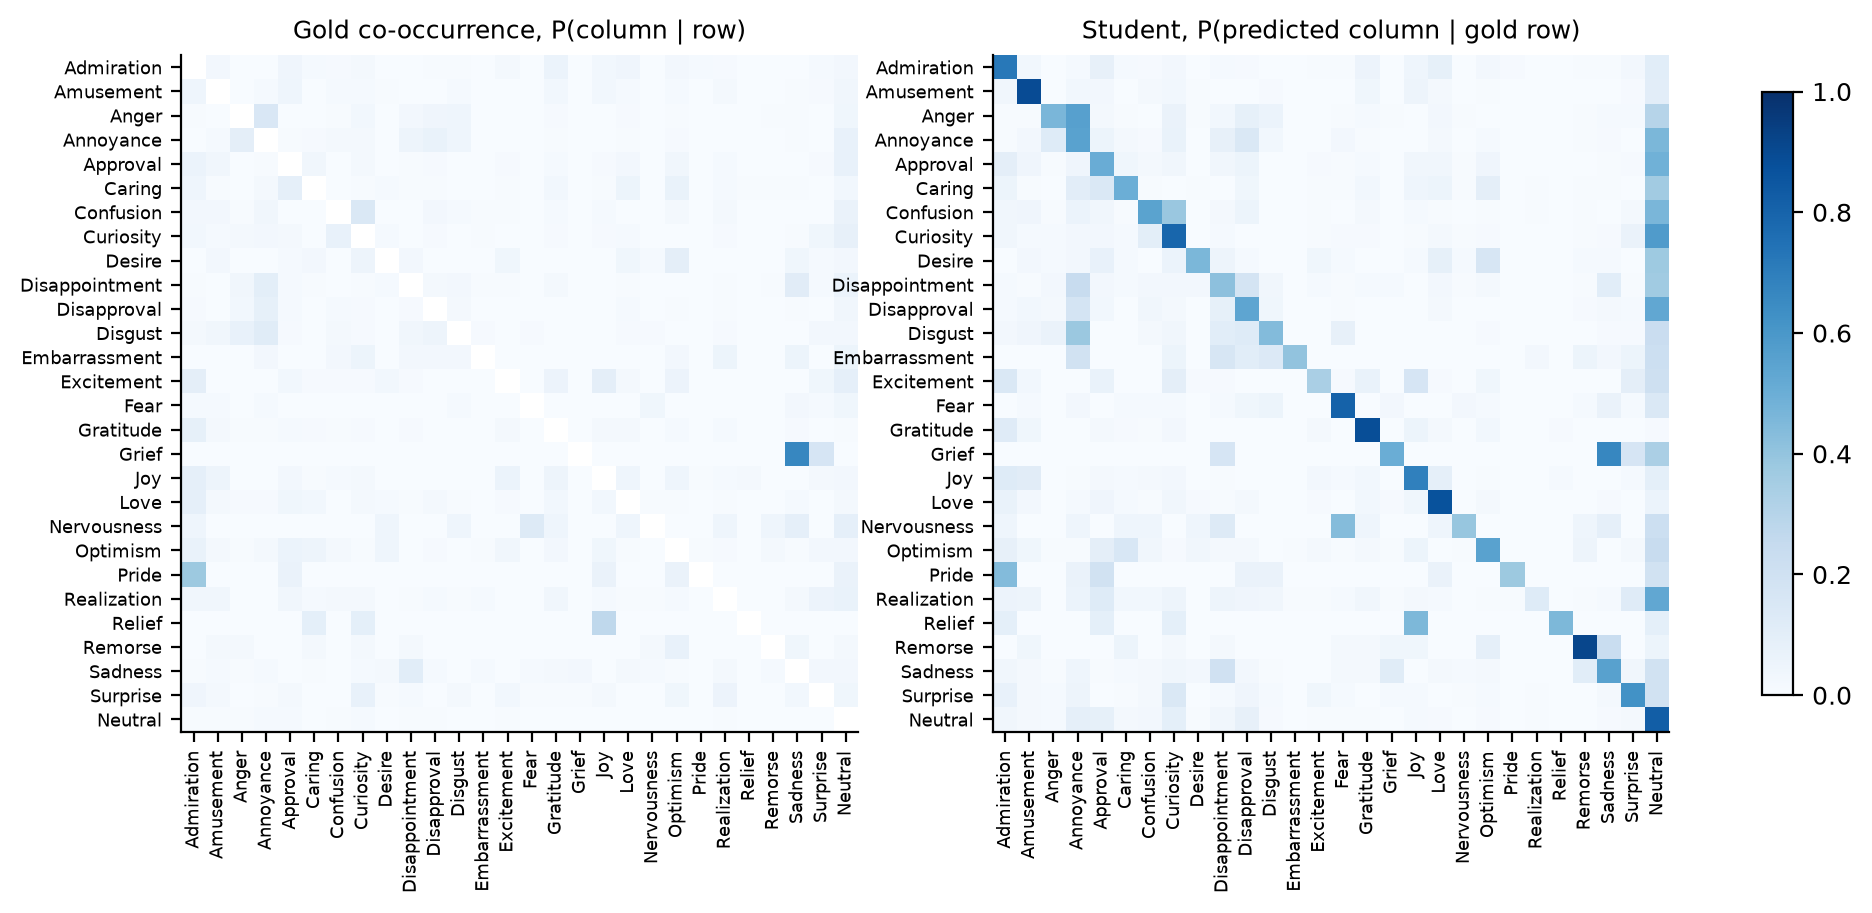
\includegraphics[width=\linewidth]{figs/cooc.png}
\caption{Left: how often label $j$ appears given label $i$ in the gold test labels (diagonal removed). Right:
how often the student predicts label $j$ for comments whose gold labels include $i$.}
\label{fig:cooc}
\end{figure}

\subsection{Ekman Groups and Out-of-Domain Transfer}

\begin{table}[H]
\centering\small
\begin{tabular}{lrrr}
\toprule
Group & \tabin tables/ekman_head.tex  \\
\midrule
\tabin tables/ekman.tex 
\bottomrule
\end{tabular}
\caption{Per-group test F1 on the Ekman view.}
\label{tab:ekman}
\end{table}

On the coarse Ekman view (Table~\ref{tab:ekman}) all transformers reach 0.63--0.66 macro-F1, just above the
paper's 0.64. Disgust is the weakest group, it is a single fine label with 793 training examples and the student predicts annoyance for 38\% of disgust comments (vs 44\% disgust).

The OOD test is the most interesting column of Table~\ref{tab:main}. Without seeing a single tweet, the
transformers get 62--63\% accuracy on dair-ai/emotion. TF-IDF falls to 45\%, which makes sense since its
features are Reddit-specific words and character patterns. The BiGRU reaches 59\%, so pretrained embeddings
already transfer quite well. Interestingly, the large teachers are not better here than the student (0.621 vs
0.632). For comparison, models trained directly on that dataset reach about 93\%, so there is a big domain
gap: the tweets are lowercase without punctuation, and most of them are written in an ``i feel ...'' style that
GoEmotions does not have.

\subsection{Calibration}
\label{sec:cal}

\begin{table}[H]
\centering\small
\begin{tabular}{lrrrrr}
\toprule
& & \multicolumn{2}{c}{ECE, all pairs} & \multicolumn{2}{c}{ECE, $p>0.05$} \\
\cmidrule(lr){3-4}\cmidrule(lr){5-6}
Model & $T$ & Raw & Scaled & Raw & Scaled \\
\midrule
\tabin tables/ece.tex 
\bottomrule
\end{tabular}
\caption{Test calibration before and after temperature scaling.}
\label{tab:ece}
\end{table}

Plain BCE fine-tuning gives well calibrated models (the BCE teacher has $T=1.02$ and ECE 0.004), so temperature
scaling has nothing to fix there. The ASL teacher is the opposite. Its focusing term pushes probabilities
towards the middle, so the raw ECE is 0.214 and the fitted temperature is 0.32 (the logits need to be sharpened
by 3$\times$). Scaling brings ECE down to 0.062, but a single temperature cannot fully repair it.

This also affected distillation. The student's soft targets were the plain average of the two teachers'
logits, and the ASL logits are on a much smaller scale, so the targets were softer than intended. The distilled
student ends up under-confident ($T=0.72$, Figure~\ref{fig:rel}). I only noticed this after training. For the
ensemble row in the table I average temperature-scaled logits instead. For the ensemble itself this hardly
matters (0.547 vs 0.550 macro-F1 for the plain average, both within noise, and after a final temperature both are
reasonably calibrated), but for distillation the scale of the targets matters more. With more GPU time I would
redistill from the calibrated average.

\begin{figure}[H]
\centering
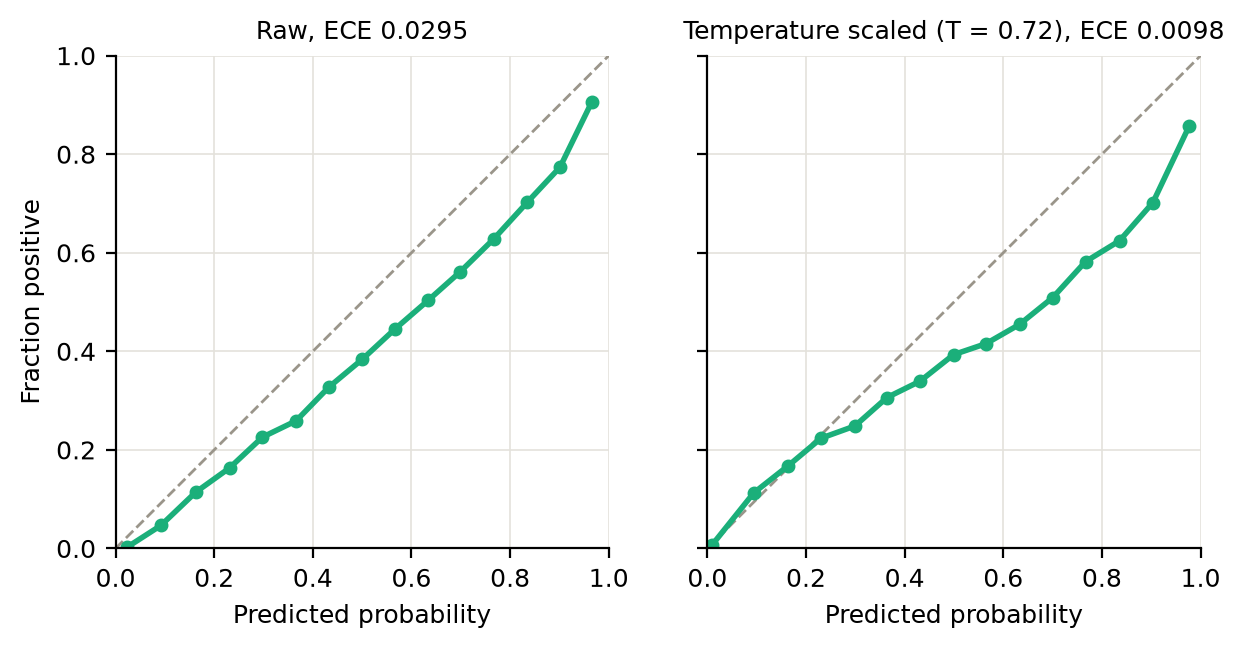
\includegraphics[width=0.8\linewidth]{figs/reliability.png}
\caption{Reliability diagram of the KD student on the test set (bins with fewer than 50 pairs hidden).}
\label{fig:rel}
\end{figure}

Figure~\ref{fig:rel} shows a limitation of a single temperature. Before scaling the student is
under-confident at the low end and over-confident from 0.3 upwards. $T=0.72$ fixes the low end, which holds
most of the pairs and therefore dominates ECE, but makes the middle range more over-confident. Per-label
temperatures or isotonic regression would probably do better. I kept one temperature because the demo
mostly shows probabilities near the thresholds, and there the scaled model is within a few points.

\subsection{Size, Speed and Quantization}

\begin{figure}[H]
\centering
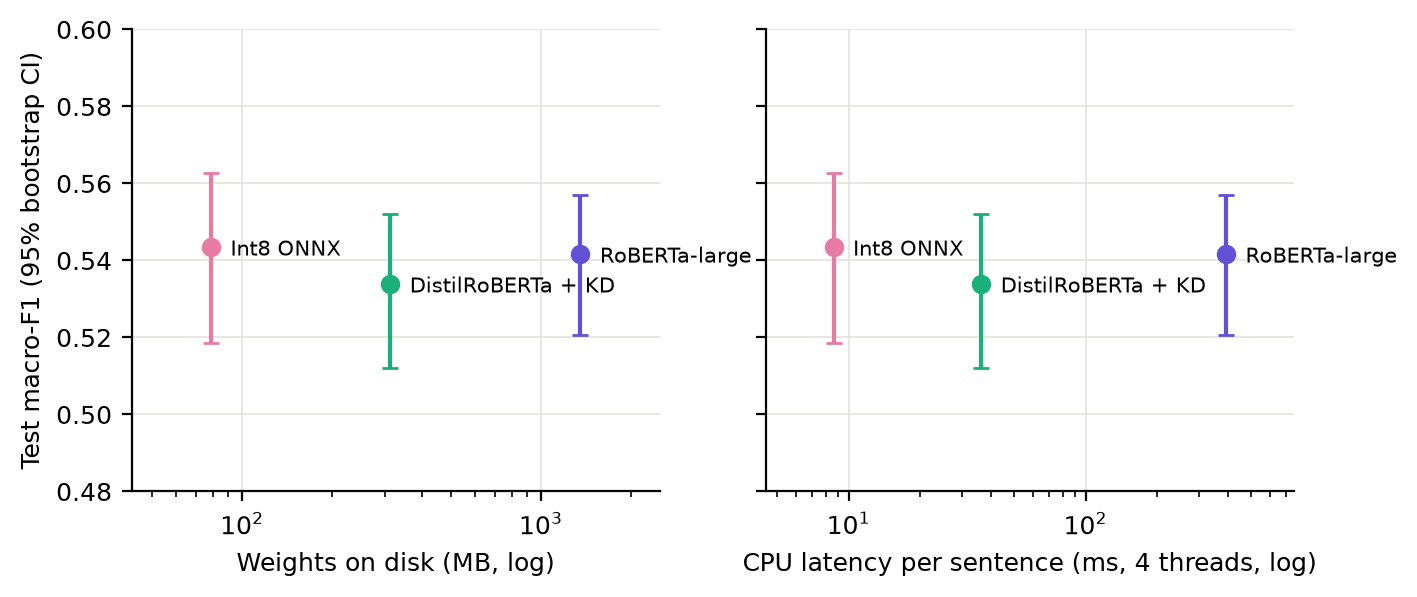
\includegraphics[width=0.85\linewidth]{figs/tradeoff.png}
\caption{Test macro-F1 against size and single-sentence CPU latency (4 threads, median over 200 test
sentences).}
\label{fig:trade}
\end{figure}

\begin{table}[H]
\centering\small
\begin{tabular}{lrrr}
\toprule
Model & Params & Size (MB) & CPU latency (ms) \\
\midrule
RoBERTa-large teacher, PyTorch fp32 & 355M & 1356 & 392 \\
DistilRoBERTa student, PyTorch fp32 & 82M & 313 & 36.3 \\
Student, ONNX fp32 & 82M & 313 & 19.0 \\
Student, ONNX int8 (deployed) & 82M & 79 & 8.6 \\
\bottomrule
\end{tabular}
\caption{Model size and latency on a laptop CPU.}
\label{tab:bench}
\end{table}

The deployed model is 17$\times$ smaller and 45$\times$ faster than one teacher (Table~\ref{tab:bench},
Figure~\ref{fig:trade}) for no measurable loss in macro-F1. The fp32 ONNX export matches PyTorch to
$3\cdot10^{-6}$ and the fp16 one to $4\cdot10^{-3}$. Int8 changes individual logits by up to 0.5 on the parity
sentences, which sounds like a lot but only moves test macro-F1 by 0.001 with fixed thresholds. In the browser
(WASM, int8) one sentence takes about 85--100\,ms including tokenization and messaging, and the word-level
explanation (one extra forward pass per word, batched in groups of 16) adds a few hundred milliseconds for a
typical sentence.

\begin{figure}[H]
\centering
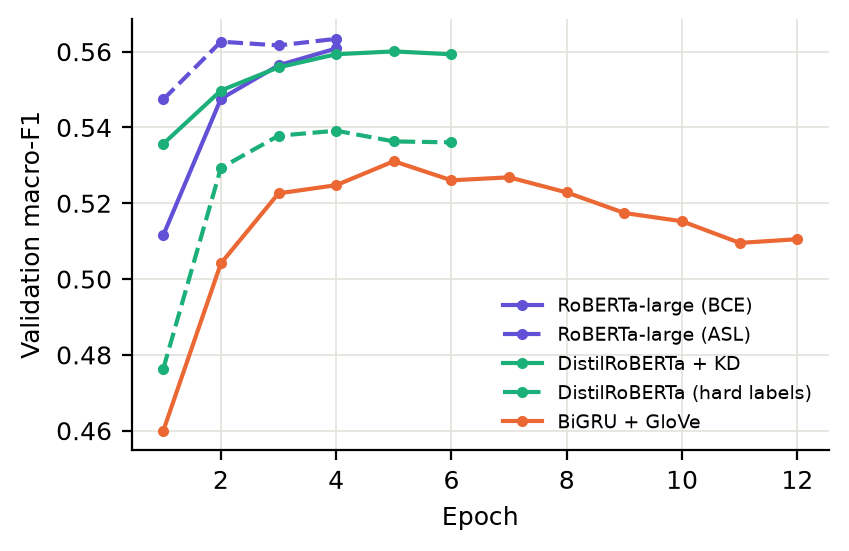
\includegraphics[width=0.55\linewidth]{figs/curves.png}
\caption{Validation macro-F1 per epoch (thresholds tuned on validation, so these are optimistic).}
\label{fig:curves}
\end{figure}

\section{The Demo}

The demo page runs the int8 student with transformers.js in a web worker. It uses WebGPU with the fp16 model
when the browser has it and WASM with the int8 model otherwise. Results update as you type (250\,ms debounce).
It shows a plain-language verdict, all 28 calibrated probabilities as bars with each label's threshold marked,
an Ekman wheel (one sector per group, member labels as spokes) and a word-level explanation. The explanation is
occlusion: the text is re-run with each word deleted, and words are shaded by how much the log-odds of the
selected emotion drop. I first used probability differences, but for a saturated prediction (gratitude at
99.9\%) deleting ``thank'' barely moved the probability and nothing was shaded, so log-odds work much better.
The ``emotion arc'' mode splits a longer text into sentences and plots the strongest emotions across them, which
is fun on chat logs. It also shows the main weakness quickly: in a diary example, the sarcastic ``great start.''
is read as admiration.

One practical problem was that the demo pages are cross-origin isolated (needed for multithreaded WASM), and
Chrome then refuses to start a worker whose script is served without the same embedder policy. The fix was to
send the header on the static chunks too.

\section{Discussion and Limitations}

\begin{itemize}
\itemsep0.2em
\item The differences between the transformer variants (BCE vs ASL teacher, teacher vs student) are within
the noise of the test set. The only small-model change that clearly helped was distillation. A proper
comparison would need several seeds per configuration, which did not fit in the free GPU budget.
\item Per-label thresholds give up to +0.04 macro-F1 over a fixed 0.5, more than any single modelling
change, but they are fragile for rare labels. Smoothing helped. Pooling validation and cross-validated
thresholds would be the next step.
\item The KD soft targets mixed two logit scales (Section~\ref{sec:cal}). Distilling from calibrated teachers is an easy
fix that I did not get to.
\item The models see Reddit only. On tweets they keep a reasonable 63\% accuracy, but the gap to in-domain
models (93\%) shows that the domain matters a lot. Sarcasm is not handled at all.
\item GoEmotions labels are noisy themselves: the paper reports that raters often disagree, and several
confusions in Figure~\ref{fig:cooc} are pairs that also co-occur in the gold labels.
\end{itemize}

\section{How to Run}

\begin{verbatim}
cd projects/06-emotion-classification
uv sync && uv run pytest -q
bash scripts/colab.sh               # training, on a GPU (or colab/train.ipynb)
uv run python -m emo.tfidf          # everything below runs on CPU
hf download manasrpandya/goemotions-runs --repo-type dataset --local-dir runs
uv run python -m emo.evaluate
uv run python -m emo.export && uv run python -m emo.evaluate
uv run python -m emo.bench && uv run python -m emo.figs
uv run python -m emo.tables
cd report && tectonic report.tex
\end{verbatim}

The tests cover the label mappings, threshold and calibration logic, dataset collation shapes, a forward pass
of a tiny randomly initialised RoBERTa and ONNX parity for it, without downloading anything.

\begin{thebibliography}{9}
\small
\bibitem{goemotions} D.~Demszky, D.~Movshovitz-Attias, J.~Ko, A.~Cowen, G.~Nemade, S.~Ravi. GoEmotions: A
Dataset of Fine-Grained Emotions. ACL 2020.
\bibitem{ekman} P.~Ekman. An Argument for Basic Emotions. Cognition and Emotion, 6(3--4), 1992.
\bibitem{asl} T.~Ridnik, E.~Ben-Baruch, N.~Zamir, A.~Noy, I.~Friedman, M.~Protter, L.~Zelnik-Manor. Asymmetric
Loss for Multi-Label Classification. ICCV 2021.
\bibitem{hinton} G.~Hinton, O.~Vinyals, J.~Dean. Distilling the Knowledge in a Neural Network. NeurIPS Deep
Learning Workshop, 2015.
\bibitem{guo} C.~Guo, G.~Pleiss, Y.~Sun, K.~Q.~Weinberger. On Calibration of Modern Neural Networks. ICML 2017.
\bibitem{glove} J.~Pennington, R.~Socher, C.~D.~Manning. GloVe: Global Vectors for Word Representation. EMNLP
2014.
\bibitem{roberta} Y.~Liu et al. RoBERTa: A Robustly Optimized BERT Pretraining Approach. arXiv:1907.11692, 2019.
\bibitem{distilbert} V.~Sanh, L.~Debut, J.~Chaumond, T.~Wolf. DistilBERT, a Distilled Version of BERT: Smaller,
Faster, Cheaper and Lighter. NeurIPS EMC$^2$ Workshop, 2019.
\bibitem{optimum} Hugging Face. Optimum: Hardware Optimization Tools for Transformers.\\
\url{https://github.com/huggingface/optimum}
\end{thebibliography}

\end{document}
